% -*- latex -*-
%%%%%%%%%%%%%%%%%%%%%%%%%%%%%%%%%%%%%%%%%%%%%%%%%%%%%%%%%%%%%%%%
%%%%%%%%%%%%%%%%%%%%%%%%%%%%%%%%%%%%%%%%%%%%%%%%%%%%%%%%%%%%%%%%
%%%%
%%%% This text file is part of the source of 
%%%% `Parallel Programming in MPI and OpenMP'
%%%% by Victor Eijkhout, copyright 2012-9
%%%%
%%%% petsc.tex : petsc stuff
%%%%
%%%%%%%%%%%%%%%%%%%%%%%%%%%%%%%%%%%%%%%%%%%%%%%%%%%%%%%%%%%%%%%%
%%%%%%%%%%%%%%%%%%%%%%%%%%%%%%%%%%%%%%%%%%%%%%%%%%%%%%%%%%%%%%%%

\Level 0 {Distributed objects}

Before we go into detail on vectors and matrices, we discuss how PETSc
treats distributed objects.

For a matrix or vector you need to specify the size. This can be done two ways:
\begin{itemize}
\item you specify the global size and PETSc distributes the object over the processes, or
\item you specify on each process the local size
\end{itemize}
If you specify both the global size and the local sizes, PETSc will check for consistency.

For example, if you have a vector of $N$ components, or a matrix of $N$
rows, and you have $P$ processes, each process will receive $N/P$
components or rows if $P$ divides evenly in~$N$. If $P$ does not divide
evenly, the excess is spread over the processes.

The way the distribution is done is by contiguous blocks: with 10
processes and 1000 components in a vector, process 0 gets the range
$0\cdots99$, process 1 gets $1\cdots199$, et cetera. This simple scheme suffices for
many cases, but PETSc has facilities for more sophisticated load
balancing.

Once an object has been created and distributed, you do not need to
remember the size or the distribution yourself: you can query these
with calls such as \lstinline{VecGetSize},
\lstinline{VecGetLocalSize}, and \lstinline{VecGetOwnershipRange}.

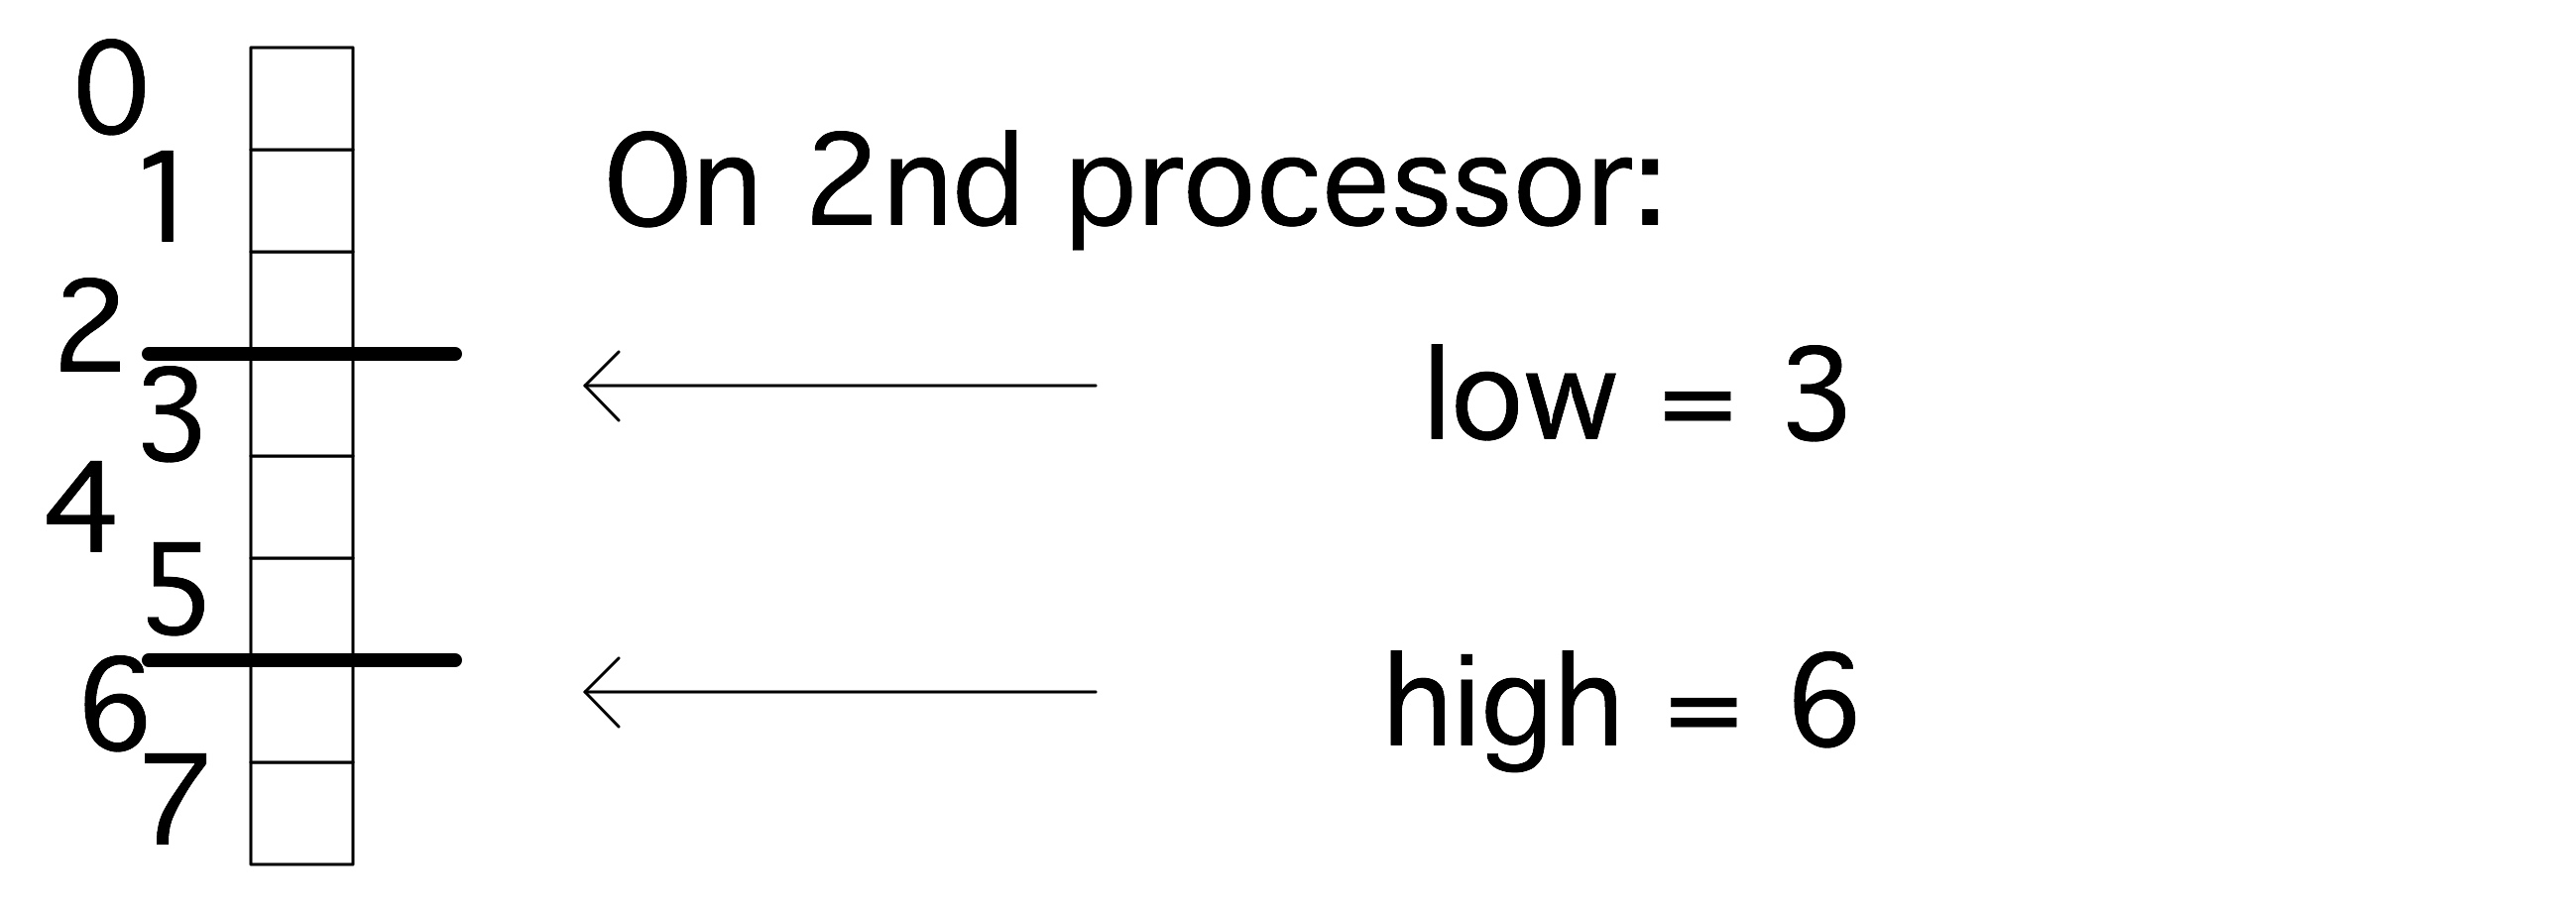
\includegraphics[scale=.1]{veclayout}

The
corresponding matrix routines \lstinline{MatGetSize},
\lstinline{MatGetLocalSize} give both information for the
distributions in $i$ and~$j$ direction, which can be
independent. Since a matrix is distributed by rows,
\lstinline{MatGetOwnershipRange} only gives a row range.

\Level 0 {Vectors}

Vectors are objects with a linear index. The elements of a vector are
floating point numbers or complex numbers (see
section~\ref{sec:petsc-complex}), but not integers: for that see
section~\ref{sec:petsc-is}.

\Level 1 {Vector construction}

Constructing a vector takes a number of steps. First of all, it needs
to be created on a communicator:
%
\petscRoutineRef{VecCreate}

\begin{pythonnote}
  In python, \n{PETSc.Vec()} creates an object with null handle, so a
  subsequent \n{create()} call is needed.
  %
  In C and Fortran, the vector type is a keyword; in Python it is a
  member of \n{PETSc.Vec.Type}.
\end{pythonnote}

The corresponding \indexpetscref{VecDestroy} destroy call deallocates data and zeros
the pointer.
%
%\petscRoutineRef{VecDestroy}

The vector type needs to be set with \indexpetscref{VecSetType}.
%
%\petscRoutineRef{VecSetType}

The most common vector types are:
\begin{itemize}
\item \indexpetscshow{VECSEQ} for sequential vectors, that is, living on a single process;
\item \indexpetscshow{VECMPI} for a vector distributed over the communicator.
\end{itemize}

Next in the creation process the vector size is set with \indexpetscref{VecSetSize}.
Since a
vector is typically distributed, this involves the global size and the
sizes on the processors. Setting both is redundant, so it is possible
to specify one and let the other be computed by the library.
%
%\petscRoutineRef{VecSetSize}

The size is queried with \indexpetscref{VecGetSize}.
%
%\petscRoutineRef{VecGetSize}

\Level 1 {Vector operations}

There are many routines operating on vectors that you would
use to write scientific applications. For instance:
%
\petscRoutineRef{VecNorm}

For debugging purpoases,
the \indexpetscref{VecView} routine can be used to display vectors on screen as
ascii output,
%
%\petscRoutineRef{VecView}
%
but the routine call also use more general \n{Viewer} objects, for
instance to dump a vector to file.

\Level 1 {Vector elements}

Setting elements of a traditional array is simple. Setting elements of
a distributed array is harder. In PETSc this is solved by having a
function \indexpetscref{VecSetValue} for setting elements that uses global numbering; any
process can set any elements in the vector:
%
%\petscRoutineRef{VecSetValue}

There is also a routine \indexpetscref{VecSetValues} for setting
multiple elements. This is mostly useful for setting dense subblocks
of a block matrix.

Using \lstinline{VecSetValue} for specifying a local vector element
corresponds to simple insertion in the local array. However,
an element that belongs to another process needs to be
transferred. This done in two calls: \indexpetscref{VecAssemblyBegin}
and \indexpetscshow{VecAssemblyEnd}.

(If you know the MPI library, you'll recognize that the first call corresponds to
posting non-blocking send and receive calls; the second then contains
the wait calls.)

Since the vector routines cover a large repertoire of operations, you
hardly ever need to access the actual elements. Should you still need
those elements, you can use \indexpetscref{VecGetArray} for general
access or \indexpetscxref{VecGetArrayRead}{VecGetArray} for read-only.

PETSc insists that you properly release this pointer again with
\indexpetscref{VecRestoreArray} or
\indexpetscxref{VecRestoreArrayRead}{VecRestoreArray}.

Note that in a distributed running context you can only get the array
of local elements. Accessing the elements from another process
requires explicit communication.

\begin{lstlisting}
PetscScalar *in_array,*out_array;
VecGetArrayRead(in,&in_array);
VecGetArray(out,&out_array);
VecGetLocalSize(in,&localsize);
for (int i=0; i<localsize; i++)
  out_array[i] = 2*in_array[i];
VecRestoreArrayRead(in,&in_array);
VecRestoreArray(out,&out_array);
\end{lstlisting}

\Level 0 {Matrices}

PETSc matrices come in a number of types, sparse and dense being the
most important ones. Another possibility is to have the matrix in
operation form, where only the action $y\leftarrow Ax$ is defined.

\Level  1 {Matrix creation}

Creating a matrix also start out with specifying a communicator:
%
\petscRoutineRef{MatCreate}

Just as with vectors, there is a local and global size; except that
that now applies to rows and columns.
%
\petscRoutineRef{MatSetSizes}
%
\petscRoutineRef{MatSizes}

There are a number of matrix types. The main choices are between
sequential versus distributed and dense versus sparse:
%
\petscRoutineRef{MatSetType}

Those four types are: \n{MATMPIDENSE} \n{MATMPIAIJ} \n{MATSEQDENSE} \n{MATSEQAIJ}.

\Level 1 {Nonzero structure}

In case of a dense matrix, once you have specified the size and the
number of MPI ranks, it is simple to determine how much space PETSc
needs to allocate for the matrix. For a sparse matrix this is more
complicated, since the matrix can be anywhere between completely empty
and completely filled in. It would be possible to have a dynamic
approach where, as elements are specified, the space grows; however,
repeated allocations and re-allocations are inefficient. For this
reason PETSc puts a small burden on the programmer: you need to
specify a bound on how many elements the matrix will contain.

We explain this by  looking at some cases. In the case of a
tridiagonal matrix you would specify that each row has three elements:

\begin{verbatim}
MatSeqAIJSetPreallocation(A,3, NULL);
\end{verbatim}

In case of a distributed matrix you need to specify this bound with
respect to the block structure of the matrix: how many non-zeros
couple between variables on the process, vs how many couple to
variables on a different process:

\begin{verbatim}
MatMPIAIJSetPreallocation(A, 3, NULL, 2, NULL);
\end{verbatim}

Specifying such bounds is often enough, and not too wasteful. However,
if many rows have fewer nonzeros than these bounds, a lot of space is
wasted. In that case you can replace the NULL arguments by an array
that lists for each row the number of nonzeros in that row.

\petscRoutineRef{MatSetPreallocation}

\Level 1 {Matrix elements}

You can set a single matrix element, or a block of them, where you
supply a set of $i$~and~$j$ indices:
%
\petscRoutineRef{MatSetValue}

After setting matrix elements, the matrix needs to be assembled. This
is where PETSc moves matrix elements to the right processor, if they
were specified elsewhere.
%
\petscRoutineRef{MatAssemblyBegin}

PETSc sparse matrices are very flexible: you can create them empty and
then start adding elements. However, this is very inefficient in
execution since the \ac{OS} needs to reallocate the matrix every time
it grows a little. Therefore, PETSc has calls for the user to indicate
how many elements the matrix will ultimately contain.
%

\begin{verbatim}
MatSetOption(A, MAT_NEW_NONZERO_ALLOCATION_ERR, PETSC_FALSE)
\end{verbatim}

If you absolutely need access to the matrix elements, there are routines

\begin{lstlisting}
MatGetRow
MatGetArray
\end{lstlisting}

PETSc insists that you properly release this pointer again:

\begin{lstlisting}
MatRestoreRow
MatRestoreArray
\end{lstlisting}

Note that in a distributed running context you can only get the array of local elements.

\Level 0 {Shell matrices}

In many scientific applications, a matrix stands for some operator,
and we are not intrinsically interested in the matrix elements, but
only in the action of the matrix on a vector. In fact, under certain
circumstances it is more convenient to implement a routine that
computes the matrix action than to construct the matrix explicitly.

Maybe surprisingly, solving a linear system of equations can be
handled this way. The reason is that PETSc's iterative solvers
(section~\ref{sec:petsc-ksp}) only need the matrix-times-vector (and perhaps
the matrix-transpose-times-vector) product.

PETSc supports this mode of working. The routine \indexpetscref{MatCreateShell}
%
%\petscRoutineRef{MatCreateShell}
%
declares the argument to be a matrix given in operator form.
The next step is then to add the custom multiplication routine, which
will be invoked by \indexpetscshow{MatMult}:
%
\petscRoutineRef{MatShellSetOperation}

The routine that implements the actual product should have the same
prototype as \indexpetscshow{MatMult}, accepting a matrix and two
vectors. The key to realizing your own product routine lies in the
`context' argument to the create routine. With
\indexpetscref{MatShellSetContext} you pass a pointer to some
structure that contains all contextual information you need. In your
multiplication routine you then retrieve this with \indexpetscref{MatShellGetContext}.

Setting the context means passing a pointer (really: an address) to
some allocated structure
\begin{lstlisting}
struct matrix_data mystruct;
MatShellSetContext( A, &mystruct );
\end{lstlisting}

The routine prototype
has this argument as a \lstinline{void*} but it's not necessary to
cast it to that. Getting the context means that a pointer to your
structure needs to be set
\begin{lstlisting}
struct matrix_data *mystruct;
MatShellGetContext( A, &mystruct );
\end{lstlisting}
Somewhat confusingly, the Get routine also has a \lstinline{void*}
argument, even though it's really a pointer variable.

\Level 0 {KSP: iterative solvers}
\label{sec:petsc-ksp}

Probably the most important activity in PETSc is solving a linear
system. This is done through a solver object: an object of the class
KSP. (This stands for Krylov SPace solver.) The solution routine
\lstinline{KSPSolve} takes a matrix and a right-hand-side and gives a
solution; however, before you can call this some amount of setup is needed.

There two very different ways of solving a
linear system: through a direct method, essentially a variant of
Gaussian elimination; or through an iterative method that makes
successive approximations to the solution. In PETSc there are only
iterative methods. We will show how to achieve direct methods later.
The default linear system solver in PETSc is fully parallel, and will
work on many linear systems, but there are many settings and
customizations to tailor the solver to your specific problem.

Create a KSP object:
%
\petscRoutineRef{KSPCreate}

After this, the basic scenario is:
\begin{lstlisting}
KSP solver;
KSPSetOperators(solver,A,A);
KSPSolve(solver,rhs,sol);
\end{lstlisting}

\Level 1 {Iterative solvers}

The main solution method for linear systems
\[ ?_x\colon Ax=b \]
in PETSc is through
so-called iterative solution methods. Instead of directly computing
the solution to the system, they compute a sequence of approximations
that, with luck, converges to the true solution. Ideally, the sequence
would stop when the distance to the true solution is small enough, but
computing this is clearly not feasible. Instead, in each step the
\indextermdef{residual}
\[ r_i=Ax_i-b \]
is computed, and the iteration is stopped if this is small enough.

Since neither
solution nor solution speed is guaranteed, an iterative solver is
subject to some tolerances:
\begin{itemize}
\item a relative tolerance for when the residual has been reduced
  enough;
\item an absolute tolerance for when the residual is objectively
  small;
\item a divergence tolerance that stops the iteration if the residual
  grows by too much; and
\item a bound on the number of iterations, regardless any progress the
  process may still be making.
\end{itemize}

\petscRoutineRef{KSPSetTolerances}

Get the reason \indexmpishow{KSPSolve} stopped:
%
\petscRoutineRef{KSPGetConvergedReason}

\Level 2 {Choice of iterator}

There are many iterative methods, and it takes a few function calls to fully specify them:

\petscRoutineRef{KSPSetType}

Here are some values:
\begin{itemize}
\item \lstinline{KSPCG}: only for symmetric positive definite systems.
\item \lstinline{KSPGMRES}: a minimization method that works fairly
  generally; has high memory demands.
\item \lstinline{KSPBCGS}: a quasi-minimization method; uses less memory than GMRES.
\end{itemize}

\Level 2 {Preconditioners}

Another part of an iterative solver is the
\indextermdef{preconditioner}; think of it as an approximation to the inverse.

\begin{lstlisting}
PC prec;
KSPGetPC(solver,&prec);
PCSetType(prec,PCILU);
\end{lstlisting}

Some popular types:
\begin{itemize}
\item \lstinline{PCILU}: an approximate factorization
\item \lstinline{PCSPAI}: an approximate inverse
\item \lstinline{PCASM}: additive Schwarz method
\end{itemize}

\Level 1 {Direct solvers}

PETSc has some support for direct solvers, that is, variants of LU
decomposition. In a sequential context, the \lstinline{PCLU}
preconditioner can be use for this: a direct solver is equivalent to
an iterative method that stops after one preconditioner
application. This can be forced by specifying a KSP type of
\lstinline{KSPPREONLY}.

Distributed direct solvers are more complicated. PETSc does not have
this implemented in its basic code, but it becomes available by
configuring PETSc with the
\indexterm{scalapack} library.

You need to specify which package provides the LU factorization:

\begin{lstlisting}
PCFactorSetMatSolverType(pc, <solvertype> )
\end{lstlisting}

where solvertype can be mumps, superlu, umfpack, or a number of
others. Note that availability of these packages depends on how PETSc
was installed on your system.

\Level 1 {Control through command line options}

From the above you may get the impression that there are lots of calls
to be made to set up a PETSc linear system and solver. And what if you
want to experiment with different solvers, does that mean that you
have to edit a whole bunch of code? Fortunately, there is an easier
way to do things. If you call the routine
%
\indexpetscref{KSPSetFromOptions}
with the \lstinline{solver} as argument,
%
PETSc will look at your command line options and take those into
account in defining the solver. Thus, you can either omit setting
options in your source code, or use this as a way of quickly
experimenting with different possibilities. Example:

\begin{verbatim}
myprogram -ksp_type gmres -ksp_type_gmres_restart 20 -ksp_max_it 200 \
  -pc_type ilu -pc_type_ilu_levels 3
\end{verbatim}

\Level 0 {DMDA: distributed arrays}

\petscRoutineRef{DMDACreate2d}

\Level 0 {Options and profiling}
\label{sec:petsc-options}

\begin{pythonnote}
  In Python, do not specify the initial hyphen of an option name.
\begin{verbatim}
hasn = PETSc.Options().hasName("n")
\end{verbatim}
\end{pythonnote}

